% A LaTeX template for EXECUTIVE SUMMARY of the MSc Thesis submissions to 
% Politecnico di Milano (PoliMi) - School of Industrial and Information Engineering
%
% S. Bonetti, A. Gruttadauria, G. Mescolini, A. Zingaro
% e-mail: template-tesi-ingind@polimi.it
%
% Last Revision: October 2021
%
% Copyright 2021 Politecnico di Milano, Italy. NC-BY

\documentclass[11pt,a4paper]{article}

%------------------------------------------------------------------------------
%	REQUIRED PACKAGES AND  CONFIGURATIONS
%------------------------------------------------------------------------------
% PACKAGES FOR TITLES
\usepackage{titlesec}
\usepackage{color}

% PACKAGES FOR LANGUAGE AND FONT
\usepackage[utf8]{inputenc}
\usepackage[english]{babel}
\usepackage[T1]{fontenc} % Font encoding

% PACKAGES FOR IMAGES
\usepackage{graphicx}
\graphicspath{{Images/}} % Path for images' folder
\usepackage{eso-pic} % For the background picture on the title page
\usepackage{subfig} % Numbered and caption subfigures using \subfloat
\usepackage{caption} % Coloured captions
\usepackage{transparent}

% STANDARD MATH PACKAGES
\usepackage{amsmath}
\usepackage{amsthm}
\usepackage{bm}
\usepackage[overload]{empheq}  % For braced-style systems of equations

% PACKAGES FOR TABLES
\usepackage{tabularx}
\usepackage{longtable} % tables that can span several pages
\usepackage{colortbl}

% PACKAGES FOR ALGORITHMS (PSEUDO-CODE)
\usepackage{algorithm}
\usepackage{algorithmic}

% PACKAGES FOR REFERENCES & BIBLIOGRAPHY
\usepackage[colorlinks=true,linkcolor=black,anchorcolor=black,citecolor=black,filecolor=black,menucolor=black,runcolor=black,urlcolor=black]{hyperref} % Adds clickable links at references
\usepackage{cleveref}
\usepackage[square, numbers, sort&compress]{natbib} % Square brackets, citing references with numbers, citations sorted by appearance in the text and compressed
\bibliographystyle{unsrtnat} % You may use a different style adapted to your field

% PACKAGES FOR THE APPENDIX
\usepackage{appendix}

% PACKAGES FOR ITEMIZE & ENUMERATES 
\usepackage{enumitem}

% OTHER PACKAGES
\usepackage{amsthm,thmtools,xcolor} % Coloured "Theorem"
\usepackage{comment} % Comment part of code
\usepackage{fancyhdr} % Fancy headers and footers
\usepackage{lipsum} % Insert dummy text
\usepackage{tcolorbox} % Create coloured boxes (e.g. the one for the key-words)
\usepackage{stfloats} % Correct position of the tables

%-------------------------------------------------------------------------
%	NEW COMMANDS DEFINED
%-------------------------------------------------------------------------
% EXAMPLES OF NEW COMMANDS -> here you see how to define new commands
\newcommand{\bea}{\begin{eqnarray}} % Shortcut for equation arrays
\newcommand{\eea}{\end{eqnarray}}
\newcommand{\e}[1]{\times 10^{#1}}  % Powers of 10 notation
\newcommand{\mathbbm}[1]{\text{\usefont{U}{bbm}{m}{n}#1}} % From mathbbm.sty
\newcommand{\pdev}[2]{\frac{\partial#1}{\partial#2}}
% NB: you can also override some existing commands with the keyword \renewcommand

%----------------------------------------------------------------------------
%	ADD YOUR PACKAGES (be careful of package interaction)
%----------------------------------------------------------------------------
\usepackage{booktabs}
\usepackage{multirow}

%----------------------------------------------------------------------------
%	ADD YOUR DEFINITIONS AND COMMANDS (be careful of existing commands)
%----------------------------------------------------------------------------

\newcommand{\overbar}[1]{\mkern 1.5mu\overline{\mkern-1.5mu#1\mkern-1.5mu}\mkern 1.5mu}


% Do not change Configuration_files/config.tex file unless you really know what you are doing. 
% This file ends the configuration procedures (e.g. customizing commands, definition of new commands)
% Set the geometric layout of the document
\usepackage{geometry}
\geometry{
  top=3cm,
  left = 2.0cm,
  right = 2.0cm,
  bottom=2cm,
  headheight= 2cm,
  headsep= 0cm,
}
\raggedbottom 

% Create color bluePoli (-> manuale grafica coordinata:  https://www.polimi.it/fileadmin/user_upload/il_Politecnico/grafica-coordinata/2015_05_11_46xy_manuale_grafica_coordinata.pdf)
\definecolor{bluePoli}{cmyk}{0.4,0.1,0,0.4}

% Custom theorem environments
\declaretheoremstyle[
  headfont=\color{bluePoli}\normalfont\bfseries,
  bodyfont=\color{black}\normalfont\itshape,
]{colored}

\captionsetup[figure]{labelfont={color=bluePoli}} % Set colour of the captions
\captionsetup[table]{labelfont={color=bluePoli}} % Set colour of the captions
\captionsetup[algorithm]{labelfont={color=bluePoli}} % Set colour of the captions

\theoremstyle{colored}
\newtheorem{theorem}{Theorem}[section]
\newtheorem{proposition}{Proposition}[section]

% Enhances the features of the standard "table" and "tabular" environments.
\newcommand\T{\rule{0pt}{2.6ex}}
\newcommand\B{\rule[-1.2ex]{0pt}{0pt}}

% Algorithm description
\newcounter{algsubstate}
\renewcommand{\thealgsubstate}{\alph{algsubstate}}
\newenvironment{algsubstates}{
    \setcounter{algsubstate}{0}%
    \renewcommand{\STATE}{%
    \stepcounter{algsubstate}%
    \Statex {\small\thealgsubstate:}\space}
    }{}
    
% Custom theorem environment
\newcolumntype{L}[1]{>{\raggedright\let\newline\\\arraybackslash\hspace{0pt}}m{#1}}
\newcolumntype{C}[1]{>{\centering\let\newline\\\arraybackslash\hspace{0pt}}m{#1}}
\newcolumntype{R}[1]{>{\raggedleft\let\newline\\\arraybackslash\hspace{0pt}}m{#1}}

% Custom itemize environment
\setlist[itemize,1]{label=$\bullet$}
\setlist[itemize,2]{label=$\circ$}
\setlist[itemize,3]{label=$-$}
\setlist{nosep}

% Set separation of columns 
\setlength{\columnsep}{30pt}

% Create command for background pic
\newcommand\BackgroundPic{% Adding background picture
	\put(230,358){
		\parbox[b][\paperheight]{\paperwidth}{%
			\vfill
			\centering
			\transparent{0.4}
			\includegraphics[width=0.5\paperwidth]{raggiera_polimi.eps}%
			\vfill
}}}

% Set indentation
\setlength\parindent{0pt}

% Custom title commands
\titleformat{\section}
{\color{bluePoli}\normalfont\Large\bfseries}
{\color{bluePoli}\thesection.}{1em}{}
\titlespacing*{\section}
{0pt}{2ex}{1ex}

\titleformat{\subsection}
{\color{bluePoli}\normalfont\large\bfseries}
{\color{bluePoli}\thesubsection.}{1em}{}
\titlespacing*{\subsection}
{0pt}{2ex}{1ex}

% Custom headers and footers
\pagestyle{fancy}
\fancyhf{}
      
\fancyfoot{}
\fancyfoot[C]{\thepage} % page
\renewcommand{\headrulewidth}{0mm} % headrule width
\renewcommand{\footrulewidth}{0mm} % footrule width

\makeatletter
\patchcmd{\headrule}{\hrule}{\color{black}\hrule}{}{} % headrule
\patchcmd{\footrule}{\hrule}{\color{black}\hrule}{}{} % footrule
\makeatother

% -> Create the header
\chead[C]{
\centering
\begin{tcolorbox}[arc=0pt, boxrule=0pt, colback=bluePoli!60, width=\textwidth, colupper=white]
    \textbf{Project summary} \hfill \textbf{\author}  
\end{tcolorbox}
}

% Insert here the info that will be displayed into your Title page 
% -> title of your work
\renewcommand{\title}{Community Detection via Maximizing Modularity Function}
% -> author name and surname
\renewcommand{\author}{Mohammadamin Vahedinia}
% -> MSc course
%\newcommand{\secondcoadvisor}{Name Surname} % insert if any otherwise comment
% -> academic year
\newcommand{\experiments}{\href{https://github.com/mavahedinia/community-detection-assignment}{experiments repository link}}

%-------------------------------------------------------------------------
%	BEGIN OF YOUR DOCUMENT
%-------------------------------------------------------------------------
\begin{document}

%-----------------------------------------------------------------------------
% TITLE PAGE
%-----------------------------------------------------------------------------
% Do not change Configuration_files/TitlePage.tex (Modify it IF AND ONLY IF you need to add or delete the Co-advisors)
% This file creates the Title Page of the document
% DO NOT REMOVE SPACES BETWEEN LINES!

%\twocolumn[{\begin{@twocolumnfalse}

% \AddToShipoutPicture*{\BackgroundPic}

% \hspace{-0.6cm}\includegraphics[width=0.6\textwidth]{logo_polimi_ing_indinf.eps}

\vspace{-1mm}
\fontsize{0.3cm}{0.5cm}\selectfont \bfseries \textsc{\color{bluePoli} Summary of the Project}\\

\vspace{-0.2cm}
\Large{\textbf{\color{bluePoli}{\title}}}\\

\vspace{-0.2cm}
\fontsize{0.3cm}{0.5cm} \selectfont \bfseries Author: \textsc{\textbf{\author}}\\


% if more than one co-advisors are present:
%\vspace{-0.4cm}
%\fontsize{0.3cm}{0.5cm}\selectfont \bfseries Co-advisors: \textsc{\textbf{\firstcoadvisor}}\textsc{\textbf{\secondcoadvisor}}\\

\vspace{-0.4cm}
\fontsize{0.3cm}{0.5cm}\selectfont \bfseries Github Repository: \textsc{\textbf{
\experiments}}

\small \normalfont

\vspace{11pt}

\centerline{\rule{1.0\textwidth}{0.4pt}}

\vspace{15pt}
%\end{@twocolumnfalse}}]

\thispagestyle{plain} % In order to not show the header in the first page

%%%%%%%%%%%%%%%%%%%%%%%%%%%%%%
%%     THESIS MAIN TEXT     %%
%%%%%%%%%%%%%%%%%%%%%%%%%%%%%%

%-----------------------------------------------------------------------------
% INTRODUCTION
%-----------------------------------------------------------------------------
\section{Introduction}
\label{sec:introduction}

Community detection, or finding the structure of groups in a network, is a popular problem in analyzing any kind of networks, such as social networks, and chemical reactions networks. As there exists many partitions for a given network, one must evaluate the quality of those partitions and select the best among of them. There are many metrics (or quality functions) proposed for evaluating partitions such as CPM \cite{cpm}, maximum likelihood \cite{likelihood}, and Modularity \cite{modularity}. It is proven that last two are equivalents \cite{limodeq}. In this report, we use modularity function, which is defined as followed:

\begin{equation}
	\label{eq:modularity}
	Q = \sum^c_{i=1} \left(e_{ii} - a_i^2\right)
\end{equation}

Where $c$ is the number of communities, $e_{ij}$ corresponds to the fractions of the edges that lie between communities $i$ and $j$, and $a_i$ is fraction of the edges that start or end in $i$th community. As mentioned in the literature, maximizing this metric may lead to some unwanted consequences like the resolution limit problem \cite{reslimit, cpm} and the degeneracy problem \cite{degen}, that is, not only maximizing modularity tends to favour merging small communities, but also many partitions exist that are almost optimal. This problems can be solved by various methods, like adding a resolution parameter to the Equation \eqref{eq:modularity} or solving a multi-objective optimization problem instead \cite{reslimit}.

However, maximizing modularity is extensively used in practice. Therefore, in the following section we are going to benchmark five algorithms mentioned below based on this method using LFR generated graphs \cite{LFR}:
\begin{enumerate}
	\item Clauset-Newman-Moore - $O(md \log n) \sim O(n \log^2 n)$ \cite{CNM}
	\item Louvain - $\sim O(n)$ \cite{louvain}
	\item Leiden - $\sim O(n)$ \cite{leiden}
	\item Simulated Annealing - $\sim O(n^{3.2})$\cite{simann, simulanncom}
	\item Leading Eigenvectors - $\sim O(n^2)$ \cite{eigen}
\end{enumerate}

Clearly, there are more methods proposed in the literature, including other Evolutionary algorithms \cite{mga, eamod, genealg} which were generating promising results.

\section{Methods}
In order to measure aforementioned algorithms' performance, first we need to generate test cases, which is described in detail in the \verb|experiments.ipynb| notebook. Overall, multiple networks were created using the LFR network generation implementation in \verb|networkx| python package, taking advantage of the multiprocessing methods to optimize case generation performance. At this step, as the LFR algorithm was not robust \cite{networkxLFR} and ended up not generating desired network, the parameters were tuned.

Furthermore, the implementation of the algorithms from \verb|networkx| (CNM), \verb|igraph| (Louvain, Simulated Annealing and Leading Eigenvectors) and \verb|leidenalg| (Leiden) packages has been used for this experiments. Additionally, the \verb|normalized_mutual_info_score| function from \verb|sklearn| package was used to measure how two partitioning (expected and predicted) were similar, in a scale from 0 to 1.

It is needed to be mentioned that for using \textit{leiden} algorithm, the modularity function without \textit{resolution parameter} has been used. Also, default parameters were set for the \textit{Simulated Annealing} algorithm.

Finally, due to the limited computing resources, all experiments are limited by a timeout, i.e., processes are halted after a certain amount of time in case of not finding the solution.

\section{Conclusive Discussion}
In summary, Tables~\ref{tbl:summaryMU}, \ref{tbl:summaryN} illustrate output of the experiments for different test cases, and Figures~
\ref{fig:per-mu}, \ref{fig:per-n} visualize NMI and modularity metrics for corresponding tables.

\begin{table*}[t]
	\centering
	\caption{Algorithms' Performance for different cases where $N = 1000$ and $\textlangle k \textrangle = 10$}\label{tbl:summaryMU}
	\begin{tabular}{c|ccc|ccc|ccc}
		\multirow{2}{*}{Algorithm}&\multicolumn{3}{c|}{$\mu = 0.2$}&\multicolumn{3}{c|}{$\mu = 0.35$}&\multicolumn{3}{c}{$\mu = 0.5$}\\
		&cases&$\overbar{Q}$&$\overbar{time}$&cases&$\overbar{Q}$&$\overbar{time}$&cases&$\overbar{Q}$&$\overbar{time}$\\
		Expected&1&0.191&&5&0.315&&5&0.115&\\
		\midrule
		CNM&1&0.203&21.578&5&0.328&17.519&5&0.218&15.270\\
		Louvain&1&0.198&0.058&5&0.349&0.042&5&0.215&0.044\\
		Leiden&1&0.225&0.049&5&0.353&0.042&5&0.229&0.033\\
		SA&1&0.224&93.035&5&0.357&67.526&5&0.242&64.672\\
		LE&1&0.099&0.143&5&0.244&0.175&5&0.145&0.254\\
	\end{tabular}

	\begin{tabular}{c|ccc|ccc}
		\multirow{2}{*}{Algorithm}&\multicolumn{3}{c|}{$\mu = 0.65$}&\multicolumn{3}{c}{$\mu = 0.8$}\\
		&cases&$\overbar{Q}$&$\overbar{time}$&cases&$\overbar{Q}$&$\overbar{time}$\\
		Expected&5&0.021&&5&-0.043&\\
		\midrule
		CNM&5&0.238&15.158&5&0.209&17.967\\
		Louvain&5&0.232&0.067&5&0.202&0.036\\
		Leiden&5&0.245&0.084&5&0.217&0.091\\
		SA&5&0.262&71.017&5&0.233&77.817\\
		LE&5&0.161&0.319&5&0.132&0.270\\
	\end{tabular}
\end{table*} 

\begin{figure}[H]
	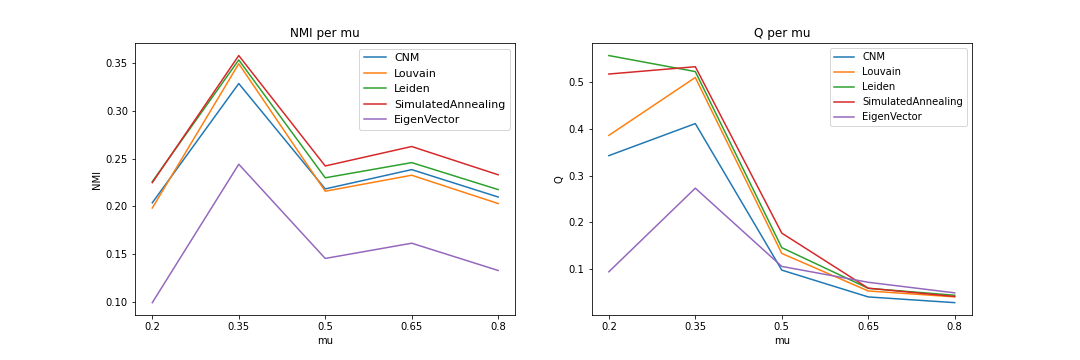
\includegraphics[width=\linewidth]{per-mu.png}
	\caption{average NMI and modularity for test cases where $N = 1000$ and $\textlangle k \textrangle = 10$}
	\label{fig:per-mu}
\end{figure}

\begin{table*}[t]
	\centering
	\caption{Algorithms' Performance for different cases where $\mu = 0.5$ and $\textlangle k \textrangle = 10$}\label{tbl:summaryN}
	\begin{tabular}{c|ccc|ccc|ccc}
		\multirow{2}{*}{Algorithm}&\multicolumn{3}{c|}{$N = 2000$}&\multicolumn{3}{c|}{$N = 3000$}&\multicolumn{3}{c}{$N = 4000$}\\
		&cases&$\overbar{Q}$&$\overbar{time}$&cases&$\overbar{Q}$&$\overbar{time}$&cases&$\overbar{Q}$&$\overbar{time}$\\
		Expected&5&0.174&&5&0.133&&5&0.184&\\
		\midrule
		CNM&5&0.218&73.214&5&0.202&168.150&5&0.228&297.048\\
		Louvain&5&0.231&0.092&5&0.196&0.224&5&0.230&0.296\\
		Leiden&5&0.241&0.154&5&0.213&0.249&5&0.246&0.322\\
		SA&4&0.219&280.97&5&0.223&486.259&5&0.251&589.507\\
		LE&5&0.131&0.630&5&0.117&1.399&5&0.138&1.986\\
	\end{tabular}
	
	\begin{tabular}{c|ccc|ccc}
		\multirow{2}{*}{Algorithm}&\multicolumn{3}{c|}{$N = 10000$}&\multicolumn{3}{c}{$N = 50000$}\\
		&cases&$\overbar{Q}$&$\overbar{time}$&cases&$\overbar{Q}$&$\overbar{time}$\\
		Expected&5&0.211&&5&0.242&\\
		\midrule
		CNM&2&0.321&822.579&\multicolumn{3}{c}{\textemdash}\\
		Louvain&5&0.260&0.320&5&0.243&2.679\\
		Leiden&5&0.293&0.329&5&0.293&2.256\\
		SA&\multicolumn{3}{c|}{\textemdash}&\multicolumn{3}{c}{\textemdash}\\
		LE&5&0.180&7.979&5&0.138&98.971\\
	\end{tabular}
\end{table*} 

\begin{figure}[H]
	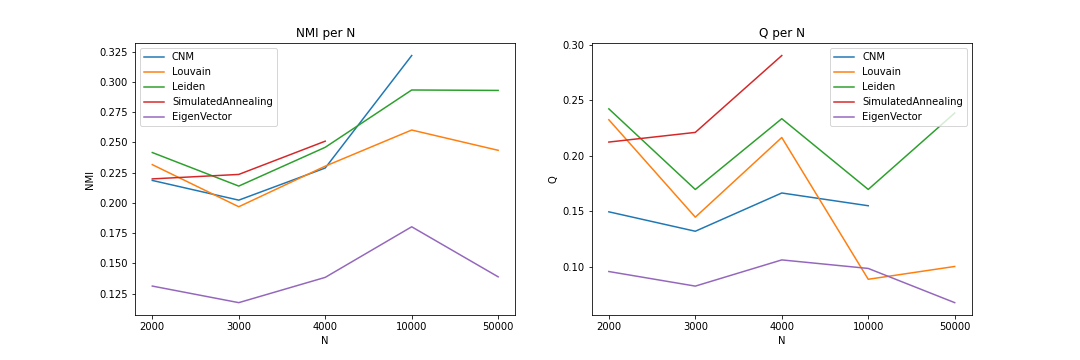
\includegraphics[width=\linewidth]{per-n.png}
	\caption{average NMI and modularity for test cases where $\mu = 0.5$ and $\textlangle k \textrangle = 10$}
	\label{fig:per-n}
\end{figure}

At a glance, from Figures~\ref{fig:per-mu} and \ref{fig:per-n} it can be inferred that Simulated Annealing method is outperforming other algorithms in both NMI and Modularity factors. However, Figure~\ref{fig:exec-time} reveals drawbacks of this algorithm regarding execution time. 

Furthermore, it can be concluded from Figure~\ref{fig:exec-time} that parameter $\mu$ does not have any significant impact on algorithms' execution time. On the other hand, according to the Figure~~\ref{fig:per-mu} increasing probability of existing extra-community links ($\mu$), decreases algorithms' performance in maximizing Modularity drastically. This phenomenon can be due to the intrinsic feature of the network.

Finally, Figure~\ref{fig:per-n} shows that by increasing size of the network, performance of the Louvain algorithm. This might be a result of the badly connected communities emerged in Louvain steps, which is guaranteed to be solved in Leiden algorithm \cite{leiden}. In spite of the fact that Leiden algorithm is derived from Louvain, Leiden does not show this pattern. Thus experimental data supports this argument.

To sum up, if $N$ (size of the network) is small enough, it is suggested to use Simulated Annealing algorithm, unless the network is not connected. In this case, Leiden has exhibited promising performance. It is also suggested to use Leiden algorithm for large networks.

\begin{figure}[H]
	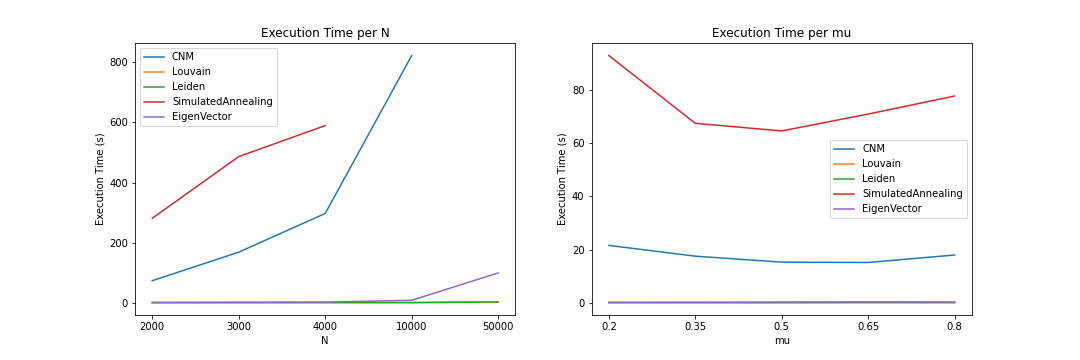
\includegraphics[width=\linewidth]{exec_time.png}
	\caption{average execution time for test cases where $\textlangle k \textrangle = 10$}
	\label{fig:exec-time}
\end{figure}


%---------------------------------------------------------------------------
%  BIBLIOGRAPHY
%---------------------------------------------------------------------------
% Remember to insert here only the essential bibliography of your work
\bibliography{bibliography.bib} % automatically inserted and ordered with this command 

\end{document}